% ============================================================
% CHAPTER 4 — METHODOLOGY
% Final M.Tech Thesis: Uncertainty-Aware Triage Learning for
% Medical Image Diagnosis: A Human-AI Collaborative Framework
% ============================================================

\chapter{METHODOLOGY}

\section{System Architecture Overview}

The proposed framework is an end-to-end pipeline that transforms raw medical images into triage decisions combining AI automation with selective human review. Figure~\ref{fig:system_architecture} presents the overall architecture, which is organised into five sequential stages: data ingestion and preprocessing, deep model inference, uncertainty quantification, triage policy execution, and evaluation.

\begin{figure}[h]
\centering
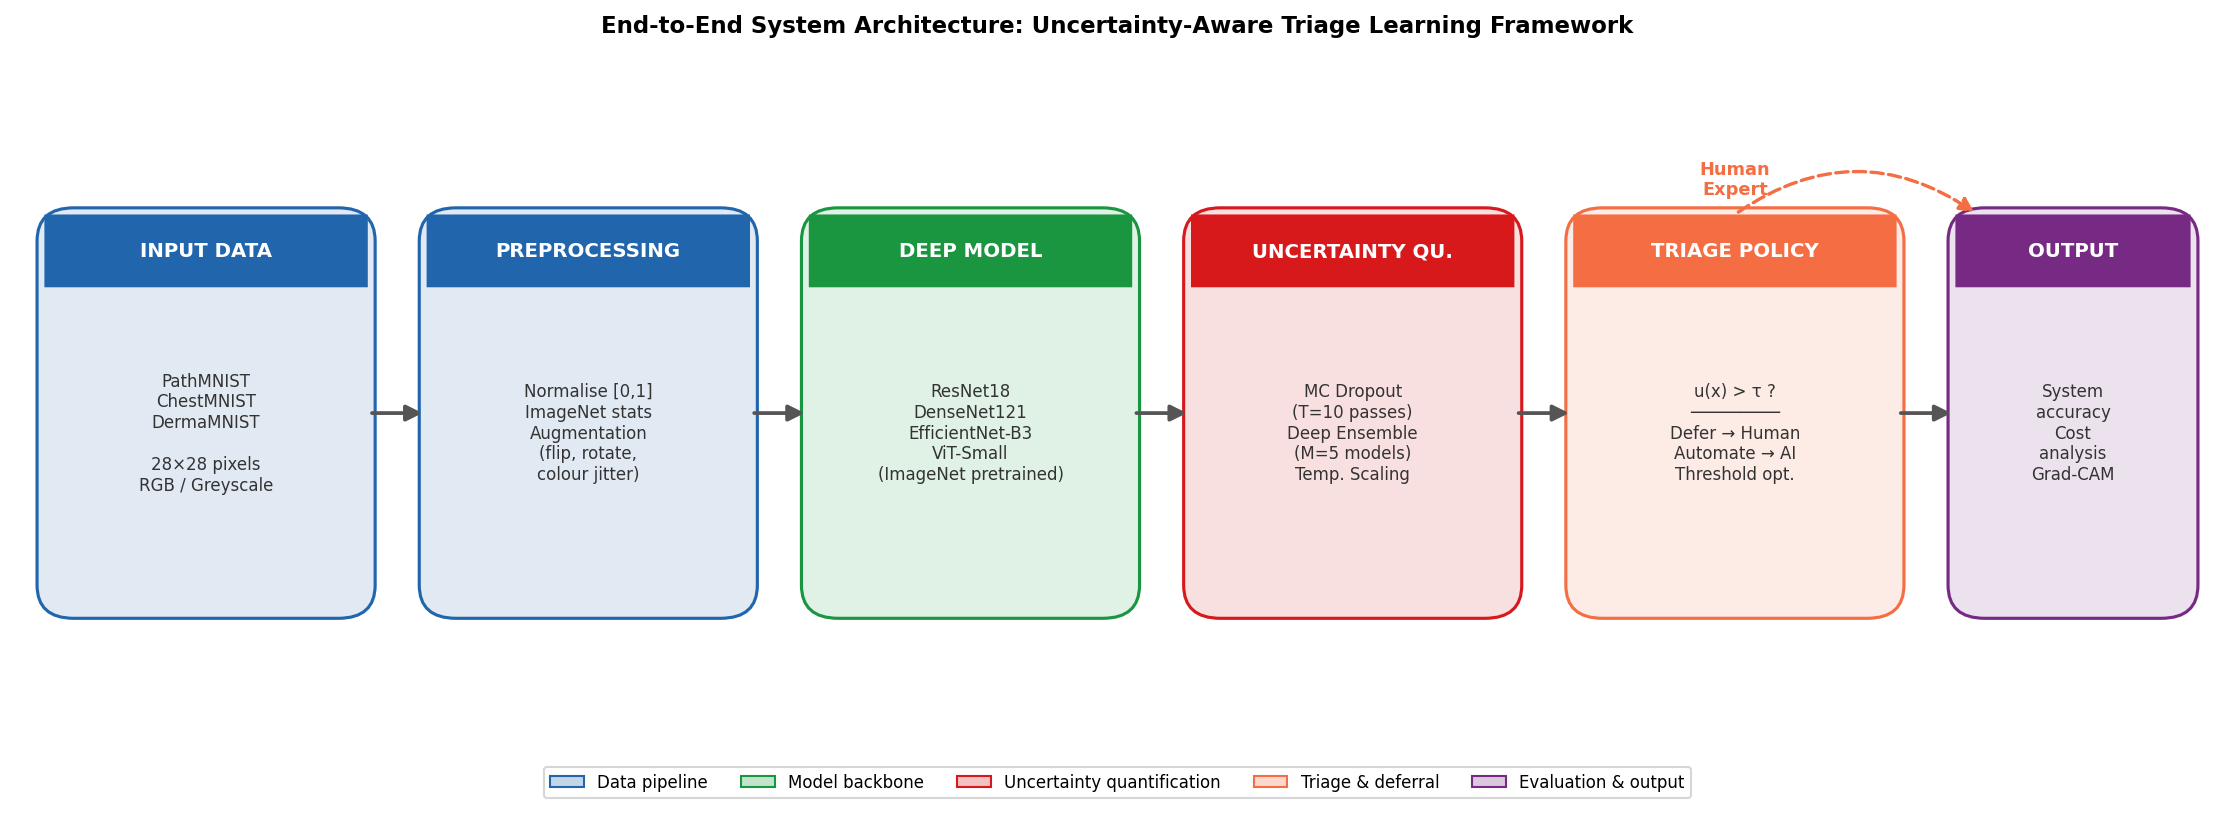
\includegraphics[width=\textwidth]{chapters/fig_system_architecture.png}
\caption{End-to-end architecture of the uncertainty-aware triage learning framework. Raw medical images pass through preprocessing, deep model inference, and uncertainty quantification before a threshold-based triage policy routes cases to either autonomous AI classification or human expert review.}
\label{fig:system_architecture}
\end{figure}

At inference time, each input image $\mathbf{x}$ is preprocessed and passed through a trained deep classifier $f_\theta$. An uncertainty quantification module produces a scalar uncertainty score $u(\mathbf{x})$ for each sample. The triage policy compares $u(\mathbf{x})$ against a learned threshold $\tau$ and either accepts the AI prediction (if $u(\mathbf{x}) \leq \tau$) or defers the case to a human reviewer (if $u(\mathbf{x}) > \tau$). The final system prediction aggregates AI decisions on automated cases with human decisions on deferred cases. Threshold selection, calibration, and Grad-CAM interpretability are all applied post-training without modifying the trained model weights.

\section{Model Architectures}

Four convolutional and transformer-based architectures are evaluated within a unified training framework. All models are initialised with ImageNet pretrained weights and fine-tuned on the target dataset. A dropout layer ($p = 0.3$) is inserted immediately before the classification head in all architectures to enable Monte Carlo Dropout inference without architectural modification.

\subsection{ResNet18}

ResNet18~\cite{he2016deep} is the primary baseline architecture. It consists of four residual stages with basic block units (two $3 \times 3$ convolution layers per block with a shortcut connection), yielding 11.2 million parameters. The residual connection in each block is defined as:
\begin{equation}
    \mathbf{y} = \mathcal{F}(\mathbf{x}, \{W_i\}) + \mathbf{x}
\end{equation}
where $\mathcal{F}(\mathbf{x}, \{W_i\})$ represents the stacked convolutional layers and $\mathbf{x}$ is the identity shortcut. The final classification head replaces the original 1000-class linear layer with a layer of size $d_{\text{feat}} \to C$, where $d_{\text{feat}} = 512$ for ResNet18 and $C$ is the number of target classes. ResNet18 is selected as the primary model for PathMNIST due to its well-understood behaviour, fast training time, and compatibility with layer-wise learning rate schedules.

\subsection{DenseNet121}

DenseNet121~\cite{huang2017densely} employs dense connectivity: each layer $l$ receives concatenated feature maps from all preceding layers within a dense block, $\mathbf{x}_l = H_l([\mathbf{x}_0, \mathbf{x}_1, \ldots, \mathbf{x}_{l-1}])$, where $[\cdot]$ denotes channel-wise concatenation. This promotes feature reuse and alleviates the vanishing gradient problem with fewer parameters than comparably deep ResNets. DenseNet121 contains 7.98 million parameters with a growth rate of 32. The final feature dimension before the classification head is 1024. Dense connectivity is particularly advantageous when training data is limited, making DenseNet121 a natural choice for DermaMNIST.

\subsection{EfficientNet-B3}

EfficientNet-B3~\cite{tan2019efficientnet} is constructed by compound scaling of a mobile-inverted bottleneck (MBConv) baseline architecture. Each MBConv block applies depth-wise separable convolutions with a squeeze-and-excitation (SE) attention module that recalibrates channel-wise feature responses:
\begin{equation}
    \tilde{\mathbf{x}} = \sigma(W_2 \cdot \text{ReLU}(W_1 \cdot \text{GAP}(\mathbf{x}))) \odot \mathbf{x}
\end{equation}
where $\text{GAP}$ denotes global average pooling and $\odot$ is channel-wise multiplication. EfficientNet-B3 has 12 million parameters and a final feature dimension of 1536. Its superior accuracy-to-FLOP ratio makes it well-suited to ChestMNIST, where the large dataset size rewards a more expressive architecture.

\subsection{ViT-Small}

ViT-Small~\cite{dosovitskiy2020image} divides the input image into non-overlapping patches of size $P \times P$ pixels, linearly projects each patch to a $D$-dimensional embedding, and prepends a learnable class token $\mathbf{z}_{\text{cls}}$. Positional embeddings are added to preserve spatial order. The sequence is processed by $L$ Transformer encoder layers, each consisting of multi-head self-attention (MSA) and a feed-forward network (FFN):
\begin{align}
    \mathbf{z}'_l &= \text{MSA}(\text{LN}(\mathbf{z}_{l-1})) + \mathbf{z}_{l-1} \\
    \mathbf{z}_l  &= \text{FFN}(\text{LN}(\mathbf{z}'_l)) + \mathbf{z}'_l
\end{align}
The final class token representation $\mathbf{z}_{\text{cls}}^L$ is passed to the classification head. For 28$\times$28 images, patches of size $4 \times 4$ are used, yielding a sequence of 49 patch tokens. ViT-Small has $D=384$, $L=12$ layers, and 6 attention heads, with 21.7 million parameters. It is evaluated on DermaMNIST where global colour context provides a complementary inductive bias to the local texture focus of CNNs.

\subsection{Training Configuration}

A unified training protocol is applied across all architectures and datasets. Table~\ref{tab:training_config} summarises the key hyperparameters.

\begin{table}[h]
\footnotesize
\centering
\caption{Training Hyperparameters Applied to All Architectures}
\label{tab:training_config}
\begin{tabular}{lll}
\toprule
\textbf{Hyperparameter} & \textbf{Value} & \textbf{Rationale} \\
\midrule
Optimiser               & AdamW                                   & Adaptive LR with weight decay \\
Weight decay            & $10^{-4}$                               & L2 regularisation \\
LR — pretrained layers  & $10^{-4}$                               & Prevent forgetting \\
LR — classifier head    & $10^{-3}$                               & Faster head adaptation \\
LR schedule             & 5-e warmup + cos annealing              & Stable convergence \\
Minimum LR              & $10^{-6}$                               & Cosine floor \\
Max epochs              & 100                                     & Sufficient for convergence \\
Batch size              & 64                                      & GPU memory / noise balance \\
Early stopping patience & 15 epochs (val loss)                    & Prevent overfitting \\
Dropout rate            & $p = 0.3$ (pre-classifier)              & Regularisation + MC Dropout \\
Random seed             & 42                                      & Reproducibility \\
\bottomrule
\end{tabular}
\end{table}

The cosine annealing schedule follows $\eta_t = \eta_{\min} + \frac{1}{2}(\eta_{\max} - \eta_{\min})(1 + \cos(\pi t / T))$, where $T = 100$ epochs and $\eta_{\min} = 10^{-6}$. The 5-epoch linear warmup raises the learning rate from 0 to $\eta_{\max}$ before handing over to the cosine schedule, preventing instability in early training due to large gradient updates on the randomly initialised classification head.

\section{Uncertainty Quantification via Monte Carlo Dropout}

\subsection{Theoretical Basis}

Gal and Ghahramani~\cite{gal2016dropout} showed that a neural network with dropout applied at every layer is equivalent, under the Bernoulli approximation, to a deep Gaussian process with a specific covariance function. Training the network with dropout minimises the KL divergence between the variational distribution $q_\phi(\boldsymbol{\theta})$ and the true posterior $p(\boldsymbol{\theta} \mid \mathcal{D})$. At test time, performing $T$ stochastic forward passes with dropout active corresponds to drawing $T$ samples from the variational posterior and computing a Monte Carlo estimate of the predictive distribution.

\subsection{Implementation}

For input $\mathbf{x}$, the $t$-th stochastic forward pass with dropout mask $\mathbf{m}_t \sim \text{Bernoulli}(1-p)$ applied to the pre-classifier layer produces:
\begin{equation}
    \hat{\mathbf{p}}_t = \text{softmax}\!\left(f(\mathbf{x};\, \boldsymbol{\theta},\, \mathbf{m}_t)\right), \quad t = 1, \ldots, T
\end{equation}
The mean prediction and three uncertainty measures are computed from the $T$-sample ensemble:
\begin{align}
    \bar{\mathbf{p}} &= \frac{1}{T} \sum_{t=1}^{T} \hat{\mathbf{p}}_t \label{eq:mean_pred} \\
    H[\bar{\mathbf{p}}] &= -\sum_{c=1}^{C} \bar{p}_c \log \bar{p}_c \quad \text{(predictive entropy)} \label{eq:entropy} \\
    \text{Var}(p_c) &= \frac{1}{T} \sum_{t=1}^{T} (p_{t,c} - \bar{p}_c)^2 \quad \text{(predictive variance)} \label{eq:var} \\
    u_{\text{conf}}(\mathbf{x}) &= 1 - H[\bar{\mathbf{p}}] / \log C \quad \text{(normalised confidence)} \label{eq:conf}
\end{align}
Predictive entropy $H[\bar{\mathbf{p}}]$ is used as the primary uncertainty score $u(\mathbf{x})$ for triage decisions, as it summarises uncertainty across the entire predicted distribution rather than focusing on a single class. The number of forward passes is set to $T = 10$ throughout, balancing uncertainty estimate quality against inference latency ($\approx 50\,\text{ms}$ per image at 5 ms per pass on a single GPU).

The model must be in training mode (\texttt{model.train()}) during MC Dropout inference to keep dropout layers active; gradient computation is disabled with \texttt{torch.no\_grad()} to avoid unnecessary memory use.

\section{Deep Ensembles for Uncertainty Estimation}

\subsection{Method}

A deep ensemble of $M = 5$ independently trained models $\{f_{\theta^{(m)}}\}_{m=1}^{M}$ is constructed by training five instances of the same architecture with different random seeds, yielding different random initialisations and different stochastic augmentation sequences. Each model produces a softmax prediction $\hat{\mathbf{p}}^{(m)} = \text{softmax}(f_{\theta^{(m)}}(\mathbf{x}))$. The ensemble mean prediction and uncertainty are:
\begin{align}
    \bar{\mathbf{p}}_{\text{ens}} &= \frac{1}{M} \sum_{m=1}^{M} \hat{\mathbf{p}}^{(m)} \label{eq:ens_mean} \\
    u_{\text{ens}}(\mathbf{x}) &= H[\bar{\mathbf{p}}_{\text{ens}}] = -\sum_c \bar{p}_c^{\text{ens}} \log \bar{p}_c^{\text{ens}} \label{eq:ens_entropy}
\end{align}
The Jensen-Shannon divergence between ensemble member predictions provides an alternative measure of epistemic uncertainty:
\begin{equation}
    \text{JSD} = H[\bar{\mathbf{p}}_{\text{ens}}] - \frac{1}{M}\sum_{m=1}^{M} H[\hat{\mathbf{p}}^{(m)}]
\end{equation}
which decomposes total uncertainty into epistemic uncertainty ($\text{JSD}$) and mean aleatoric uncertainty ($\frac{1}{M}\sum_m H[\hat{\mathbf{p}}^{(m)}]$).

\subsection{Comparison with MC Dropout}

Deep ensembles and MC Dropout are compared along four dimensions: accuracy of the mean prediction, calibration quality (ECE/MCE), uncertainty-error AUROC, and computational overhead. Ensembles incur a $5\times$ training cost and $5\times$ inference latency compared to a single model, but do not require dropout during training and thus do not impose the Bayesian interpretation constraints that MC Dropout assumes. They are therefore used as a higher-quality reference against which MC Dropout is benchmarked.

\section{Probability Calibration — Temperature Scaling}

\subsection{Motivation}

Modern deep neural networks are systematically overconfident~\cite{guo2017calibration}: the maximum softmax probability $\max_c \hat{p}_c$ tends to be higher than the empirical frequency of correct predictions at that confidence level. Overconfidence inflates the predicted confidence of both correct and incorrect predictions, compressing the uncertainty score distribution and degrading triage performance — high-confidence errors that should be deferred are instead automated.

\subsection{Temperature Scaling Procedure}

Temperature scaling~\cite{guo2017calibration} applies a scalar parameter $T > 0$ to the model's logit vector $\mathbf{z}$ before the softmax:
\begin{equation}
    \hat{\mathbf{p}}_T = \text{softmax}(\mathbf{z} / T)
\end{equation}
For $T > 1$, the distribution is softened (confidence reduced); for $T < 1$, it is sharpened. The optimal temperature $T^*$ is found by minimising the negative log-likelihood on the validation set:
\begin{equation}
    T^* = \arg\min_{T > 0} \; -\frac{1}{N_{\text{val}}} \sum_{i=1}^{N_{\text{val}}} \log \hat{p}_{T,y_i}(\mathbf{x}_i)
\end{equation}
This is a one-dimensional convex optimisation problem solved with L-BFGS in a single pass over the validation set. Temperature scaling does not alter class-level accuracy (argmax is invariant to uniform rescaling of logits) but modifies confidence magnitudes and thereby changes the distribution of entropy-based uncertainty scores. The impact on ECE, reliability diagrams, and triage threshold selection is evaluated empirically in Chapter~5.

\section{Triage Policy and Deferral Mechanism}

\subsection{Threshold-Based Deferral}

The triage policy is a threshold-based deferral rule. For sample $i$ with uncertainty score $u_i = H[\bar{\mathbf{p}}_i]$ and threshold $\tau$, the deferral indicator is:
\begin{equation}
    d_i = \mathbb{I}(u_i > \tau)
\end{equation}
where $\mathbb{I}(\cdot)$ is the indicator function. The deferral rate and automation rate are:
\begin{equation}
    \text{DR}(\tau) = \frac{1}{N}\sum_{i=1}^{N} d_i, \qquad \text{AR}(\tau) = 1 - \text{DR}(\tau)
\end{equation}

\subsection{Human Expert Simulation}

In the absence of real clinical annotators, human expert performance is modelled probabilistically. For a deferred sample $i$, a simulated human with accuracy $p_h$ predicts the correct label with probability $p_h$ and uniformly draws from the remaining $C-1$ classes with probability $(1-p_h)/(C-1)$ per incorrect class:
\begin{equation}
    \hat{y}_i^h = \begin{cases} y_i & \text{with probability } p_h \\ \text{Uniform}(\mathcal{Y} \setminus \{y_i\}) & \text{with probability } 1 - p_h \end{cases}
\end{equation}
Human accuracy is evaluated at four levels: $p_h \in \{0.80, 0.90, 0.95, 0.99\}$, representing general clinical staff, trained technicians, specialist pathologists/dermatologists, and expert subspecialists respectively. For multi-label ChestMNIST, $p_h$ is applied independently per label.

\subsection{System Prediction and Accuracy}

The final system prediction combines AI and human decisions:
\begin{equation}
    \hat{y}_i^{\text{sys}} = d_i \cdot \hat{y}_i^h + (1 - d_i) \cdot \hat{y}_i^{\text{AI}}
\end{equation}
System accuracy decomposes additively:
\begin{equation}
    \text{Acc}_{\text{sys}}(\tau) = \text{AR}(\tau) \cdot \text{Acc}_{\text{AI}}(\tau) + \text{DR}(\tau) \cdot p_h
\end{equation}
where $\text{Acc}_{\text{AI}}(\tau)$ is the AI accuracy on the automated subset $\{i : d_i = 0\}$. As $\tau$ increases, more cases are automated and $\text{Acc}_{\text{AI}}(\tau)$ rises (since only high-confidence, low-uncertainty cases are retained), but $\text{AR}(\tau) \to 1$ eliminates the human contribution. The optimal threshold balances these opposing trends.

\section{Threshold Optimisation Strategies}

\subsection{Accuracy-Maximising Threshold}

The accuracy-optimal threshold is:
\begin{equation}
    \tau^*_{\text{acc}} = \arg\max_{\tau \in \mathcal{T}} \; \text{Acc}_{\text{sys}}(\tau, p_h)
\end{equation}
evaluated at the primary human accuracy level $p_h = 0.95$. A grid of $|\mathcal{T}| = 50$ linearly-spaced thresholds from 0 to $\max_i u_i$ is swept over the test set, computing system accuracy at each point. The threshold yielding the global maximum system accuracy is selected.

\subsection{Cost-Minimising Threshold}

The cost-optimal threshold minimises the total operational cost function defined in Section~\ref{sec:cost_model}:
\begin{equation}
    \tau^*_{\text{cost}} = \arg\min_{\tau \in \mathcal{T}} \; C_{\text{total}}(\tau)
\end{equation}
The cost-optimal threshold is generally lower than the accuracy-optimal threshold, deferring a larger fraction of cases to human review in exchange for fewer AI errors. The trade-off between the two objectives is visualised through accuracy-vs-automation-rate and cost-vs-threshold curves reported in Chapter~5.

\subsection{Sensitivity Analysis}

Both thresholds are evaluated across all four human accuracy levels $p_h \in \{0.80, 0.90, 0.95, 0.99\}$ to assess how triage benefit depends on reviewer quality. The system is additionally evaluated at the accuracy-optimal threshold for the primary $p_h = 0.95$ level across all other $p_h$ values, revealing the degradation incurred when actual human performance deviates from the assumed level used during threshold selection.

\section{Cost Modelling Framework}
\label{sec:cost_model}

\subsection{General Cost Function}

The operational cost function assigns monetary costs to two event types: AI classification errors and human review instances. For a given threshold $\tau$:
\begin{equation}
    C_{\text{total}}(\tau) = c_{\text{err}} \cdot N_{\text{err}}^{\text{AI}}(\tau) + c_{\text{rev}} \cdot N_{\text{defer}}(\tau)
\end{equation}
where $N_{\text{err}}^{\text{AI}}(\tau)$ is the number of AI errors on automated cases and $N_{\text{defer}}(\tau) = \text{DR}(\tau) \cdot N$ is the number of cases deferred to human review.

\subsection{Dataset-Specific Cost Parameters}

Error costs reflect the clinical severity of misdiagnosis in each domain. Table~\ref{tab:cost_params} specifies the cost parameters used per dataset.

\begin{table}[h]
\footnotesize
\centering
\caption{Cost Model Parameters by Dataset}
\label{tab:cost_params}
\begin{tabular}{lcccl}
\toprule
\textbf{Dataset} & $c_{\text{err}}$ & $c_{\text{rev}}$ & \textbf{Ratio} & \textbf{Rationale} \\
\midrule
PathMNIST   & \$100 & \$2  & 50:1  & Histopathology re-read cost \\
ChestMNIST  & \$200 & \$5  & 40:1  & Critical finding (e.g.\ pneumothorax) \\
DermaMNIST  & \$500 & \$5  & 100:1 & Missed melanoma mortality risk \\
\bottomrule
\end{tabular}
\end{table}

The baseline cost of operating AI-only is $C_{\text{baseline}} = c_{\text{err}} \cdot N_{\text{err}}^{\text{base}}$, where $N_{\text{err}}^{\text{base}}$ is the number of AI errors with no deferral ($\tau \to \infty$). Cost savings are reported as $\Delta C = C_{\text{baseline}} - C_{\text{total}}(\tau^*_{\text{cost}})$.

\subsection{Break-Even Analysis}

To assess robustness to cost parameter uncertainty, a break-even analysis identifies the maximum review cost $c_{\text{rev}}^{\text{max}}$ at which the triage system remains cost-beneficial relative to AI-only operation:
\begin{equation}
    c_{\text{rev}}^{\text{max}} = \frac{c_{\text{err}} \cdot (N_{\text{err}}^{\text{base}} - N_{\text{err}}^{\text{AI}}(\tau^*))}{N_{\text{defer}}(\tau^*)}
\end{equation}
If $c_{\text{rev}}^{\text{max}} \gg c_{\text{rev}}$, the economic case for deployment is robust to cost overruns.

\section{Interpretability via Grad-CAM}

\subsection{Grad-CAM Computation}

Gradient-weighted Class Activation Mapping (Grad-CAM)~\cite{selvaraju2017grad} generates a spatial saliency map $L^c \in \mathbb{R}^{H' \times W'}$ for class $c$ at the final convolutional layer with feature maps $A^k \in \mathbb{R}^{H' \times W'}$, $k = 1, \ldots, K$. The importance weight for feature map $k$ is the global average of the gradient of the class score $S^c$ with respect to $A^k$:
\begin{equation}
    \alpha_k^c = \frac{1}{H' W'} \sum_{i=1}^{H'} \sum_{j=1}^{W'} \frac{\partial S^c}{\partial A_{ij}^k}
\end{equation}
The class activation map is then the ReLU of the weighted sum of feature maps:
\begin{equation}
    L^c = \text{ReLU}\!\left(\sum_{k=1}^{K} \alpha_k^c\, A^k\right)
\end{equation}
The ReLU retains only activations that contribute positively to the class score $S^c$. The map $L^c$ is upsampled to input resolution $(28 \times 28)$ using bilinear interpolation and normalised to $[0, 1]$ before overlay on the original image.

\subsection{Visualisation Protocol}

Grad-CAM maps are generated for four categories of samples on PathMNIST and DermaMNIST:
\begin{enumerate}
    \item \textbf{Confident correct:} Low uncertainty ($u_i < Q_1$) and correct prediction.
    \item \textbf{Uncertain correct:} High uncertainty ($u_i > Q_3$) but correct prediction.
    \item \textbf{Confident error:} Low uncertainty ($u_i < Q_1$) but incorrect prediction (most clinically concerning case).
    \item \textbf{Uncertain error:} High uncertainty ($u_i > Q_3$) and incorrect prediction (correctly deferred by triage).
\end{enumerate}
For each category, five representative examples are selected and their Grad-CAM maps are visualised. The target class for gradient computation is always the predicted class $\hat{y}_i$, enabling assessment of the features the model used to arrive at its decision, regardless of correctness. For confident errors, the Grad-CAM for the true class $y_i$ is additionally computed and shown alongside the predicted-class map to reveal the discrepancy between what the model attended to and what it should have attended to.

\subsection{Qualitative Assessment Criteria}

Grad-CAM maps are assessed qualitatively against the following criteria, adapted from domain knowledge:
\begin{itemize}
    \item \textbf{PathMNIST:} Does the saliency map concentrate on cellular structures (nuclei, gland boundaries, lymphocyte clusters) rather than background staining or image artefacts?
    \item \textbf{DermaMNIST:} Does the map highlight lesion boundaries, asymmetric pigmentation patterns, or atypical vascular structures rather than uninformative skin background?
    \item \textbf{Confident errors:} Is the saliency map plausibly attributable to a confusable class (indicating a genuine ambiguity) or does it concentrate on artefactual regions (indicating a spurious correlate)?
\end{itemize}
These qualitative assessments provide actionable diagnostic insight: saliency maps focusing on artefactual regions suggest data collection or preprocessing issues that warrant investigation, while maps focusing on genuinely ambiguous morphological features indicate irreducible difficulty that motivates human deferral.
